\documentclass[11pt,a4paper]{article}

\usepackage[utf8]{inputenc}
\usepackage[T1]{fontenc}
\usepackage[spanish,es-nodecimaldot]{babel}
\usepackage{lmodern}
\usepackage{geometry}
\usepackage{microtype}
\usepackage{xcolor}
\usepackage{booktabs}
\usepackage{tabularx}
\usepackage{array}
\usepackage{enumitem}
\usepackage{fancyhdr}
\usepackage{hyperref}
\usepackage{graphicx}
\usepackage[section]{placeins}

\geometry{left=2.6cm,right=2.6cm,top=2.6cm,bottom=2.6cm}
\definecolor{Azul}{HTML}{17283B}
\definecolor{Rojo}{HTML}{B73739}
\definecolor{Gris}{HTML}{53606B}
\definecolor{Suave}{HTML}{F3F5F7}
\hypersetup{colorlinks=true,linkcolor=Azul,urlcolor=Rojo}
\setlength{\parindent}{0pt}
\setlength{\parskip}{0.55em}
\setlist[itemize]{leftmargin=1.5em,itemsep=0.2em,topsep=0.2em}
\setlist[enumerate]{leftmargin=1.6em,itemsep=0.2em,topsep=0.2em}
\renewcommand{\arraystretch}{1.18}
\newcommand{\codigo}[1]{\texttt{#1}}
\newcommand{\cita}[1]{\textsuperscript{\textcolor{Rojo}{[#1]}}}
\newcommand{\dato}[1]{\textcolor{Azul}{\bfseries #1}}
\graphicspath{{figuras/}}

\pagestyle{fancy}
\fancyhf{}
\fancyhead[L]{\small\textcolor{Gris}{Five Nights of Terror}}
\fancyhead[R]{\small\textcolor{Gris}{Avance final · IHC}}
\fancyfoot[C]{\thepage}
\renewcommand{\headrulewidth}{0.4pt}

\begin{document}

\begin{titlepage}
\thispagestyle{empty}
\begin{center}
\vspace*{1.5cm}
{\Large\bfseries Universidad Católica San Pablo\par}
\vspace{0.35cm}
{\large Curso de Interacción Humano--Computador\par}
\vspace{1.8cm}
{\color{Rojo}\rule{0.75\textwidth}{2pt}\par}
\vspace{0.55cm}
{\Huge\bfseries Avance final\par}
\vspace{0.45cm}
{\LARGE Five Nights of Terror\par}
\vspace{0.35cm}
{\large Juego de vigilancia con interacción entre PC, tablet y cámara\par}
\vspace{0.55cm}
{\color{Rojo}\rule{0.75\textwidth}{2pt}\par}
\vspace{1.8cm}
\begin{tabular}{>{\bfseries}p{3.5cm}p{8cm}}
Curso: & Interacción Humano--Computador (CS2H1)\\
Estudiantes: & Marcelo Torres y Anthony Briceño\\
Semestre: & 2026-02\\
Universidad: & Universidad Católica San Pablo\\
\end{tabular}
\vfill
{\large Arequipa, Perú · 2026\par}
\end{center}
\end{titlepage}

\section{Descripción del aplicativo}

\textit{Five Nights of Terror} es un prototipo de juego de terror y vigilancia en el que la persona debe sobrevivir desde las 12:00 a.\,m. hasta las 6:00 a.\,m. durante seis noches. La experiencia reparte la atención entre un monitor de PC, donde se ve la escena tridimensional, y una tablet, donde se resuelven minitareas y se controla la caja musical. Una cámara web permite estimar si el jugador dirige la cabeza hacia la pantalla. Si un animatrónico lo alcanza, la noche termina en derrota; al sobrevivir hasta las 6:00 a.\,m. se desbloquea la siguiente, y completar la sexta produce la victoria final.\cita{R1}

El juego propone tres presiones simultáneas. \dato{Freddy} puede avanzar cuando el jugador deja de mirar el PC; \dato{Vixy} se vuelve peligrosa cuando se acumulan tareas sin resolver; y \dato{Puppet} depende del nivel de una caja musical que se vacía con el tiempo. Cada amenaza requiere una respuesta distinta: volver la vista al monitor, completar tareas o dar cuerda a la caja desde la tablet. Esta alternancia es la mecánica central, no un efecto secundario de la interfaz.\cita{R1}

El prototipo integra componentes que antes podían ejecutarse de forma separada. En la versión examinada, Unity toma las decisiones sobre tiempo, tareas, movimiento y ataques; Flutter presenta controles y minijuegos; un relay en Python transmite mensajes entre ambos. El informe describe esa versión del proyecto. No presenta resultados de una evaluación formal con participantes, porque no consta una prueba completa de ese tipo en los materiales revisados.\cita{R1}\cita{R2}

\section{Principales características y tecnologías usadas}

\begin{itemize}
  \item \textbf{Vigilancia con cámara.} MediaPipe Unity Plugin obtiene puntos faciales y el componente \codigo{HeadOrientationTracker} calcula una proporción entre frente, nariz y mentón. El estado booleano \codigo{mirandoPC} se usa para la mecánica de Freddy y para la prueba del tutorial.\cita{R1}\cita{R4}
  \item \textbf{Escena 3D y enemigos.} Unity 2022.3.30f1 muestra el entorno, mueve los animatrónicos mediante rutas y \codigo{NavMeshAgent}, controla la caja musical y presenta las pantallas de espera y de resultado de la noche.\cita{R1}\cita{R5}
  \item \textbf{Audio ambiental.} Estática de fondo durante la partida (baja de volumen cuando suena otro efecto), \textit{My Grandfather's Clock} cuando Puppet está por salir, campanas a las 6:00 a.\,m. y música en el menú. Los sonidos pertenecen a Unity, no a la tablet.\cita{R1}
  \item \textbf{Dificultad progresiva.} Freddy tolera entre 35 s (noche 1) y 20 s (noche 6) sin ser mirado antes de avanzar; Vixy exige menos tareas pendientes para avanzar y atacar en las noches altas; y cada noche dura entre 2:00 y 2:45 minutos reales para las seis horas de juego.\cita{R1}
  \item \textbf{Tablet interactiva.} Flutter implementa el menú, el tutorial, la lista de tareas y diez minijuegos: cables, perillas, secuencia, ritmo, WiFi, ventiladores, temperatura, procesamiento de datos, subida de datos y trazado de curso. La caja musical es una acción permanente aparte de esa lista.\cita{R1}\cita{R3}
  \item \textbf{Comunicación bidireccional.} Unity y Flutter intercambian mensajes JSON mediante WebSocket. \codigo{UnityRelay} los reenvía según el rol de cada conexión; el relay no ejecuta las reglas del juego.\cita{R1}\cita{R6}
  \item \textbf{Ejecutable único.} \codigo{iniciar.sh} levanta el relay y el juego con doble clic desde un acceso directo, y apaga el relay al cerrar. La pantalla de espera muestra la IP a la que debe conectarse la tablet.\cita{R1}
  \item \textbf{Continuidad.} El progreso por noche se almacena en \codigo{PlayerPrefs}. Tras una derrota puede repetirse la noche; tras una victoria se habilita la siguiente hasta la sexta.\cita{R1}
\end{itemize}

\begin{table}[ht]
\centering
\small
\begin{tabularx}{\textwidth}{@{}p{2.6cm}X X@{}}
\toprule
Componente & Tecnología principal & Responsabilidad en el prototipo\\
\midrule
PC & Unity, C\#, MediaPipe, NavMesh & Simulación, cámara, reglas de juego, enemigos y resultados.\\
Tablet & Flutter, Dart & Menú, minitareas, caja musical y controles del tutorial.\\
Enlace local & Python y WebSocket & Reenvío de mensajes JSON entre PC y tablet.\\
\bottomrule
\end{tabularx}
\caption{Distribución de responsabilidades observada en el proyecto.}
\end{table}

\section{Diseño y arquitectura del aplicativo}

La arquitectura sigue una separación de responsabilidades. \codigo{UnityGameSessionController} mantiene el estado de la noche, genera tareas, recibe resultados y comunica ataques o victoria. \codigo{AnimatronicUnityBrain} decide el avance y las condiciones de ataque de cada enemigo; \codigo{HeadOrientationTracker} entrega el estado de mirada. En Flutter, las pantallas y widgets muestran el estado que llega desde Unity y devuelven las acciones del jugador. Esta organización evita que la tablet y el PC calculen por separado resultados contradictorios.\cita{R1}

\begin{center}
\small
\fcolorbox{Azul}{Suave}{\parbox[c][1.5cm][c]{2.6cm}{\centering\textbf{Tablet / Flutter}\\Menú, tareas y controles}}
\quad$\Longleftrightarrow$\quad
\fcolorbox{Azul}{Suave}{\parbox[c][1.5cm][c]{2.1cm}{\centering\textbf{UnityRelay}\\Mensajes JSON}}
\quad$\Longleftrightarrow$\quad
\fcolorbox{Azul}{Suave}{\parbox[c][1.5cm][c]{2.6cm}{\centering\textbf{PC / Unity}\\Reglas, escena y cámara}}
\end{center}

El flujo comienza con \codigo{connect}. Unity inicializa la noche y envía \codigo{task\_list}, \codigo{night\_status} y \codigo{estado\_puppet}. La tablet presenta estos estados y, al terminar una tarea, responde con \codigo{task\_completed} o \codigo{task\_failed}. Unity actualiza el estado de los enemigos y, cuando corresponde, publica \codigo{attack} y \codigo{game\_over}. La cámara se procesa en el PC; el intercambio entre dispositivos se basa en eventos y estados, no en transmitir el video de la webcam.\cita{R1}

Para la demostración, el juego se abre como un programa normal: el lanzador detecta si el puerto 8000 ya tiene un relay, impide abrir dos copias a la vez y apaga el relay al terminar. La IP local se calcula en Unity y se muestra en la pantalla de espera, de modo que la tablet solo necesita escribirla en Opciones. Al elegir \textit{Salir} en la tablet, Unity cierra el juego. Esta forma de arranque reemplazó el flujo anterior de levantar relay, editor y aplicación por separado.\cita{R1}

El uso de WebSocket permite que ambos extremos reciban eventos durante una sesión sin abrir una conexión nueva para cada interacción. El estándar define un canal bidireccional; en el prototipo, el contenido de cada mensaje se expresa como JSON y la lógica de negocio permanece en Unity.\cita{R6}

\section{Menú de inicio y tutorial}

El menú de la tablet ofrece \textit{Tutorial}, \textit{Nuevo juego}, \textit{Continuar}, \textit{Opciones} y \textit{Salir}. Desde Opciones se configura la conexión con el PC. La escena de Unity muestra una pantalla de espera mientras no hay partida (figura~\ref{fig:menu}). El tutorial se abre desde la tablet y presenta su contenido en el monitor; los botones \textit{Anterior}, \textit{Siguiente} y \textit{Terminar} permanecen en la tablet.\cita{R1}

\begin{figure}[htbp]
\centering
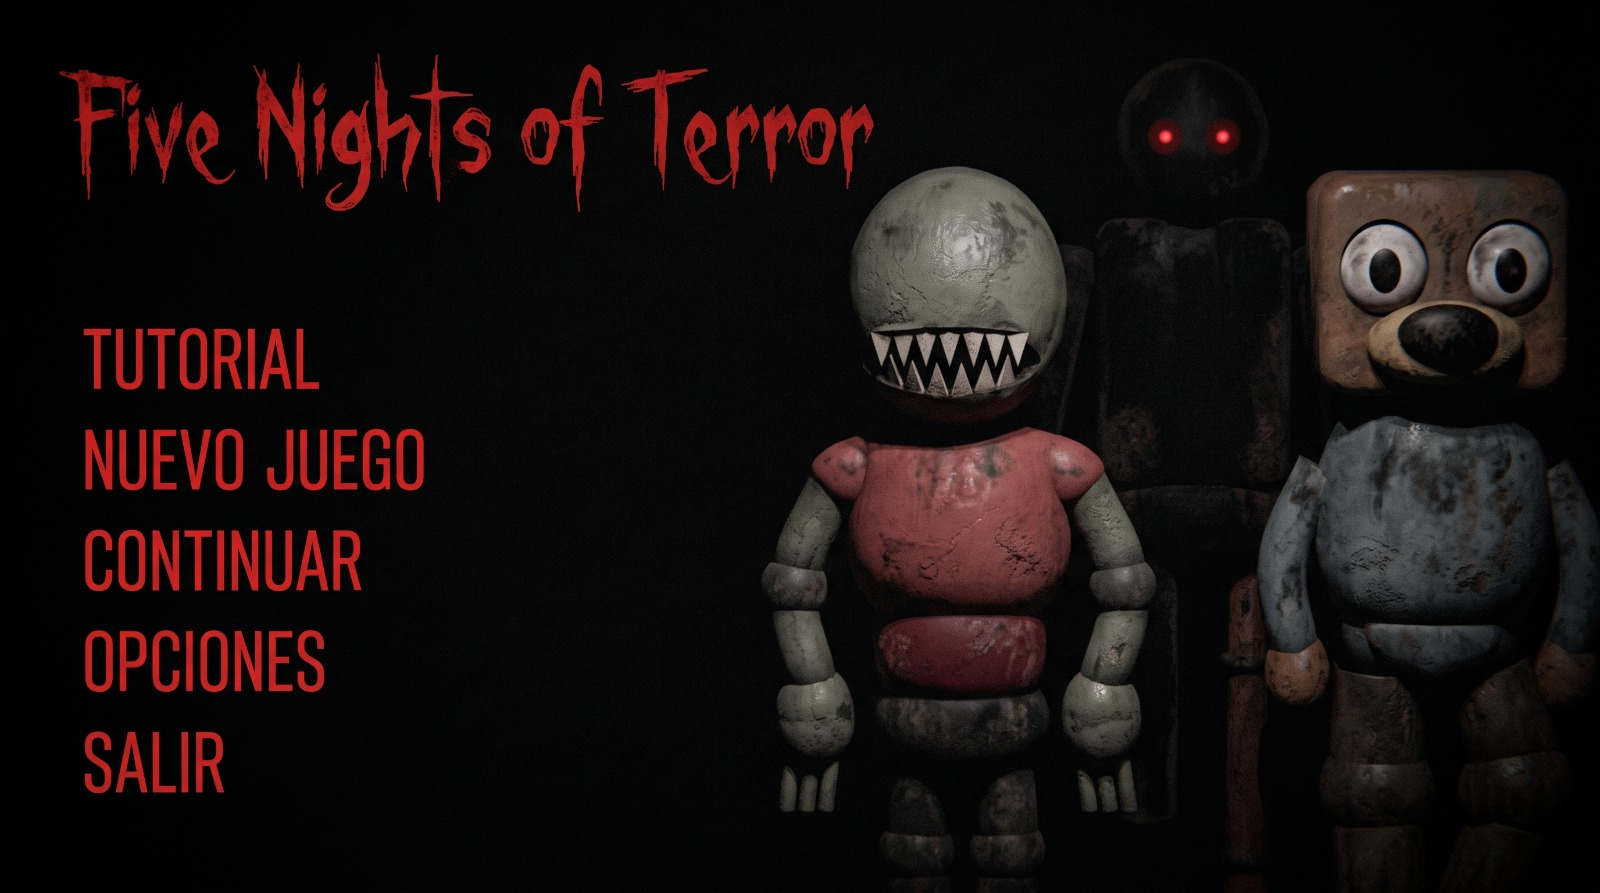
\includegraphics[width=0.8\textwidth]{menu.png}
\caption{Menú de inicio del prototipo. Captura proporcionada por los autores.}
\label{fig:menu}
\end{figure}

El tutorial actual está organizado en tres pantallas:
\begin{enumerate}
  \item \textbf{Objetivo y amenazas.} En la mitad izquierda explica cómo sobrevivir y ganar. En la mitad derecha aparecen representaciones de Freddy, Vixy y Puppet con la forma en que cada uno amenaza al jugador.
  \item \textbf{Minitareas.} Resume las diez tareas de la tablet y recuerda que la caja musical requiere atención continua.
  \item \textbf{Prueba interactiva.} La tablet abre el minijuego real de conectar cables; en el PC aparece la señal en vivo de la misma cámara usada por el juego. El jugador debe completar los cables y mantener la mirada hacia el PC durante dos segundos. El botón \textit{Terminar} se habilita cuando ambas comprobaciones se completan.\cita{R1}
\end{enumerate}

La primera pantalla presenta el objetivo de sobrevivir seis noches y explica las amenazas de Freddy, Vixy y Puppet. La segunda reúne las diez minitareas en una vista de consulta rápida, de modo que el jugador pueda reconocerlas antes de comenzar la partida (figuras~\ref{fig:tutorial-mision} y~\ref{fig:tutorial-tareas}).

\begin{figure}[htbp]
\centering
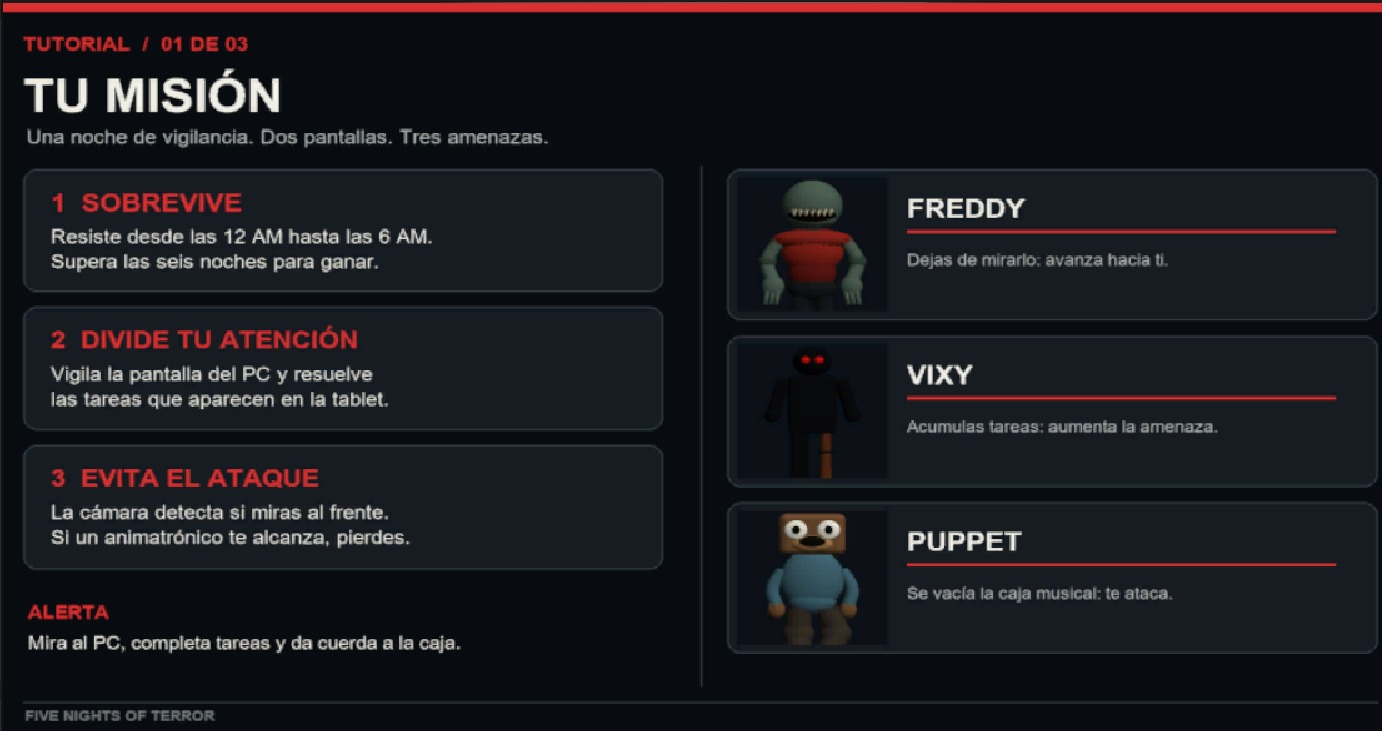
\includegraphics[width=0.96\textwidth]{tutorial_mision.png}
\caption{Primera pantalla del tutorial: misión a la izquierda y animatrónicos con sus formas de ataque a la derecha. Captura del prototipo proporcionada por los autores.}
\label{fig:tutorial-mision}
\end{figure}

\begin{figure}[htbp]
\centering
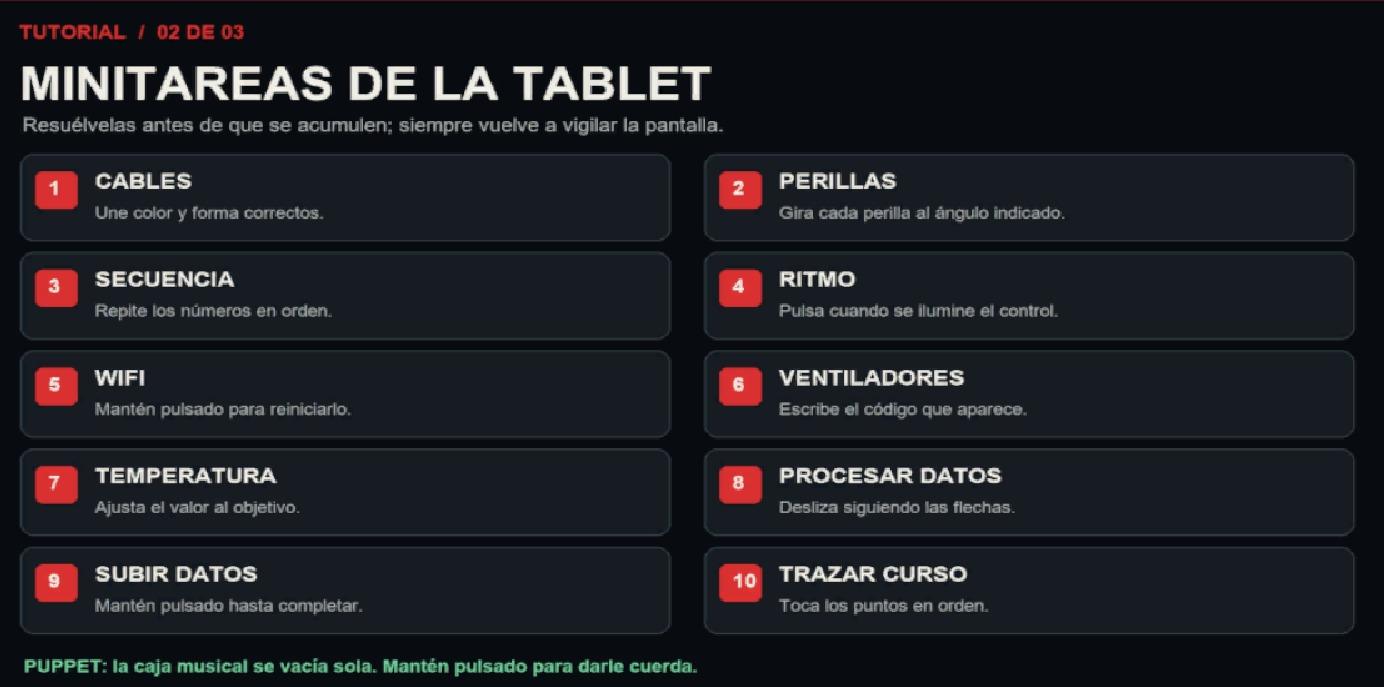
\includegraphics[width=0.96\textwidth]{tutorial_minitareas.png}
\caption{Segunda pantalla del tutorial: explicación breve de las diez minitareas y recordatorio de la caja musical. Captura del prototipo proporcionada por los autores.}
\label{fig:tutorial-tareas}
\end{figure}

En la última pantalla, el PC muestra el video de la cámara en tiempo real y el estado de la detección, mientras que la tablet ofrece la tarea real de conectar cables. Las figuras~\ref{fig:tutorial-prueba-pc} y~\ref{fig:tutorial-prueba-tablet} muestran las dos vistas simultáneas. La opción \textit{Terminar} aparece deshabilitada hasta completar los cables y verificar la mirada.

\begin{figure}[htbp]
\centering
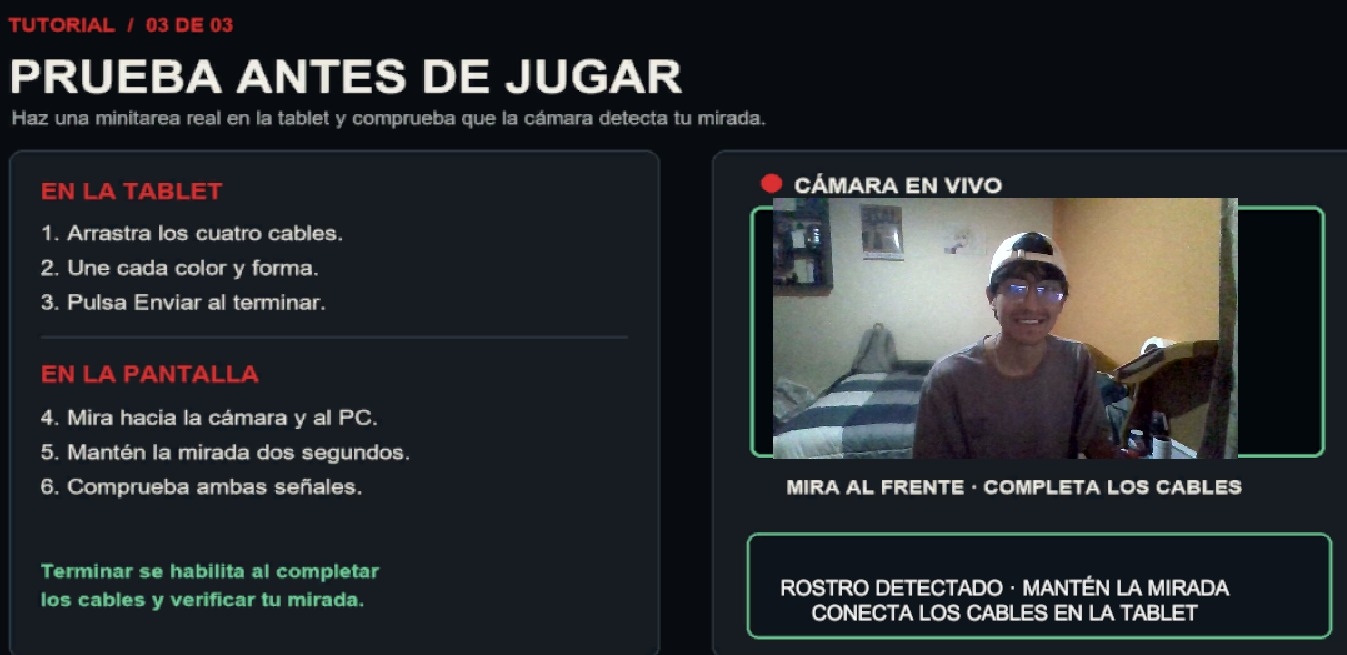
\includegraphics[width=0.96\textwidth]{tutorial_prueba_pc.png}
\caption{Tercera pantalla del tutorial en el PC: instrucciones y señal en vivo de la cámara para comprobar la mirada. Captura del prototipo proporcionada por los autores.}
\label{fig:tutorial-prueba-pc}
\end{figure}

\begin{figure}[htbp]
\centering
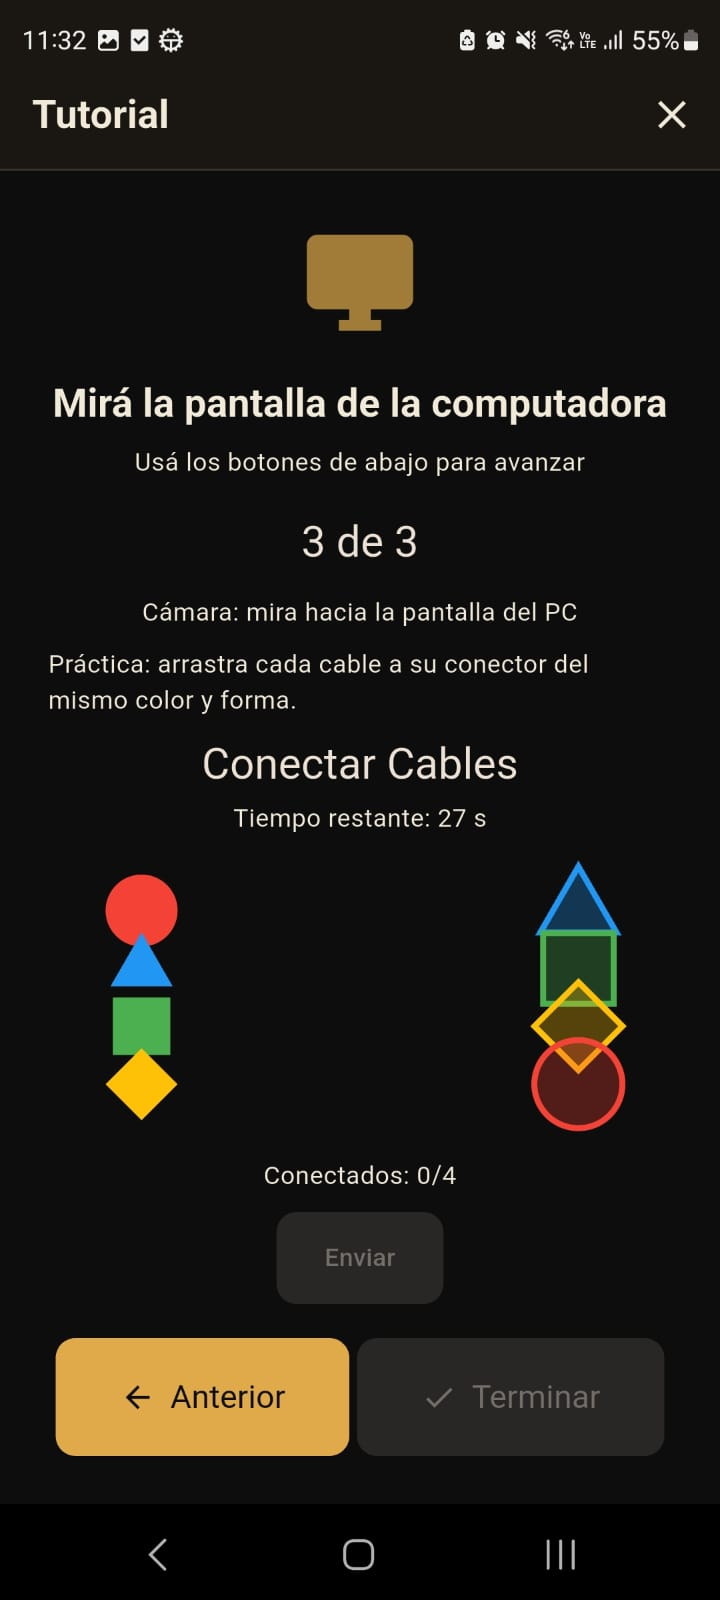
\includegraphics[height=10cm,keepaspectratio]{tutorial_prueba_tablet.png}
\caption{Tercera pantalla del tutorial en la tablet: práctica de cables con colores y formas, junto al avance de la prueba. Captura del prototipo proporcionada por los autores.}
\label{fig:tutorial-prueba-tablet}
\end{figure}

El modo tutorial reutiliza la conexión del juego, pero no inicia una noche. Unity informa el índice y el número total de pantallas mediante \codigo{tutorial\_estado}; así, la tablet puede mostrar el progreso y bloquear la navegación fuera de los extremos. La prueba final usa mensajes específicos para comunicar la tarea completada y el estado de mirada.\cita{R1}

\section{Diseño de los eventos de interacción}

Los eventos se diseñaron alrededor de la acción de la persona y la respuesta visible del sistema. La tabla distingue la entrada, el procesamiento y la retroalimentación que recibe el jugador.

\begin{table}[ht]
\centering
\footnotesize
\begin{tabularx}{\textwidth}{@{}p{2.15cm}p{3.0cm}X X@{}}
\toprule
Evento & Entrada del jugador & Respuesta del sistema & Retroalimentación\\
\midrule
Iniciar o continuar & Selección en la tablet & Unity inicia la noche elegida y genera tareas. & Estado de noche y menú de tareas.\\
Mirar el PC & Orientación del rostro ante la cámara & Se actualiza \codigo{mirandoPC}; puede detenerse Freddy. & Video de cámara y reacción del enemigo.\\
Resolver tarea & Toques, arrastres, giros o deslices & Flutter envía resultado; Unity retira o mantiene la presión de la tarea. & Confirmación del minijuego y lista actualizada.\\
Dar cuerda & Pulsación sostenida en la tablet & Se incrementa el nivel de la caja mientras dura la acción. & Indicador de la caja musical.\\
Ataque o fin & Estado de enemigos y reloj & Unity decide derrota, victoria de noche o victoria final. & Jumpscare o pantalla de resultado.\\
Tutorial & Navegación y prueba en la tablet & Unity cambia de pantalla y verifica tarea y mirada. & Progreso y estados de la prueba.\\
\bottomrule
\end{tabularx}
\caption{Eventos de interacción principales. Elaboración a partir del código del prototipo.\cita{R1}}
\end{table}

Al terminar una noche, la PC muestra una pantalla de resultado (\textit{Noche X completada}, \textit{No sobreviviste} o \textit{Turno completado} tras la sexta) que permanece hasta que la persona toca \textit{Continuar} en la tablet; en la derrota aparece tras el \textit{jumpscare}. La tablet muestra su propia pantalla de final y regresa al menú, donde se decide si continuar. No se muestran puntajes: el logro es sobrevivir.\cita{R1}

La mecánica exige alternar la atención. En cables, por ejemplo, el jugador arrastra cada pieza hasta un conector que coincide en color \emph{y forma}; después debe volver a vigilar el PC. En la caja musical se mantiene presionado un control. La información crítica debería ser perceptible incluso cuando la persona está mirando la otra pantalla, motivo por el que los avisos y su oportunidad temporal son parte del diseño de interacción.\cita{R1}\cita{R7}

\section{Análisis de especificidad y limitaciones finales}

El documento de análisis previo propone estudiar la especificidad por \textbf{dominio}, \textbf{tarea}, \textbf{dispositivo} y \textbf{usuario}, además del recorrido estímulo--percepción--decisión--respuesta. En este juego, esas dimensiones están estrechamente ligadas: la amenaza tiene sentido porque la persona debe retirar la mirada del PC para usar la tablet, y la cámara convierte esa acción en una variable del juego.\cita{R2}

\begin{table}[ht]
\centering
\small
\begin{tabularx}{\textwidth}{@{}p{2.5cm}X X@{}}
\toprule
Dimensión & Especificidad del aplicativo & Límite observado o pendiente\\
\midrule
Usuario & Jugador que puede seguir una escena 3D, manipular la tablet y situarse ante una webcam. & Hace falta definir mejor condiciones de uso y comprobarlas con personas diversas.\\
Tarea & Vigilar, decidir prioridades y resolver minijuegos con tiempo. & La carga de alternar dos pantallas puede dificultar la prioridad de acciones.\\
Dispositivo & PC, tablet, cámara y red local funcionando al mismo tiempo. & Fallas de cámara, iluminación, postura o conexión afectan la experiencia.\\
Interacción & Color, formas, movimiento, audio y gestos táctiles. & No todas las tareas tienen una alternativa equivalente al arrastre, al tiempo o al audio.\\
\bottomrule
\end{tabularx}
\caption{Síntesis de especificidad y limitaciones, actualizada respecto del análisis previo.\cita{R1}\cita{R2}}
\end{table}

\textbf{Detección de mirada.} El código usa un umbral fijo de 1,3 sobre una proporción de distancias faciales. Cuando no encuentra la malla o esta se oculta, \codigo{mirandoPC} pasa a falso. Esa regla es funcional para el prototipo, pero puede confundir una pérdida de detección con la decisión de mirar a otro lugar. También depende de la posición de la cámara, la luz y la postura. La prueba del tutorial hace visible el estado, aunque todavía no sustituye una calibración individual ni una evaluación de precisión.\cita{R1}\cita{R2}

\textbf{Accesibilidad y retroalimentación.} El análisis anterior señalaba que los cables se distinguían solo por color. La versión actual añade círculo, triángulo, cuadrado y rombo, lo que reduce esa dependencia y sigue el criterio de no comunicar información únicamente por color.\cita{R1}\cita{R2}\cita{R7} El mismo criterio se aplicó a otras tareas: en ritmo los botones llevan triángulo, círculo o cuadrado y el activo se marca con borde grueso; en perillas y secuencia el estado completado se indica con una marca de verificación; la conexión incorrecta de cables se dibuja punteada; y la urgencia de cada tarea del menú se refuerza con íconos de reloj y de alerta. El reloj de la tablet muestra solo la hora, sin minutos, para no atraer la mirada hacia la tablet.\cita{R1} Permanecen por examinar el tamaño de los blancos táctiles, el tiempo de respuesta exigido por ritmo y arrastre, el uso de pulsación sostenida, la legibilidad de prioridades y la equivalencia visual de las señales sonoras. La dependencia del audio o el potencial malestar por sustos deben explicarse al jugador y evaluarse, no asumirse como resueltos.\cita{R2}

La comparación de las figuras~\ref{fig:cables-antes} y~\ref{fig:cables-despues} documenta el cambio. En la versión anterior, cada cable y conector se diferenciaba principalmente por su color; esto dificultaba identificar parejas si los colores no se distinguían bien. Tras reconocer esa limitación, se incorporaron \textbf{formas u objetos geométricos} (círculo, triángulo, cuadrado y rombo) a los elementos que deben unirse. Ahora cada pareja se reconoce por \textbf{color y forma}, por lo que el jugador dispone de una pista visual adicional para conectar los cables con mayor facilidad. Esta mejora reduce la dependencia exclusiva del color, aunque todavía necesita una prueba de uso con jugadores para medir su efecto.

\begin{figure}[htbp]
\centering
\begin{minipage}[t]{0.46\textwidth}
\centering
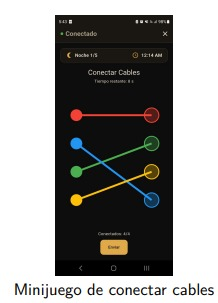
\includegraphics[width=\linewidth,height=5.5cm,keepaspectratio]{cables_solo_colores_anterior.png}
\caption{Minitarea anterior: correspondencia de cables indicada principalmente por colores. Captura proporcionada por los autores.}
\label{fig:cables-antes}
\end{minipage}\hfill
\begin{minipage}[t]{0.46\textwidth}
\centering
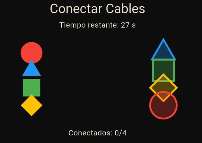
\includegraphics[width=\linewidth,height=5.5cm,keepaspectratio]{cables_formas_actual.png}
\caption{Minitarea actual: formas geométricas añadidas a los colores para identificar las parejas. Captura proporcionada por los autores.}
\label{fig:cables-despues}
\end{minipage}
\end{figure}

\textbf{Alcance de la evidencia.} Este apartado es una inspección del código y de los documentos proporcionados. No contiene porcentajes de usabilidad, precisión de mirada ni tasas de éxito de minijuegos: tales métricas requerirían sesiones instrumentadas con participantes, dispositivos y condiciones de iluminación definidos.\cita{R2}

\section{Problemas encontrados}

\begin{enumerate}
  \item \textbf{Dependencia de MediaPipe ausente en una copia del proyecto.} Los ejemplos de \codigo{Assets/MediaPipeUnity} estaban presentes, pero el paquete \codigo{com.github.homuler.mediapipe} no acompañaba esa copia. Unity inició en modo seguro y mostró errores de tipos y espacios de nombres no encontrados. Se restauró una copia completa del paquete 0.16.3 desde otra instalación del mismo proyecto, tras lo cual el usuario confirmó que el proyecto volvió a ejecutarse. Esta incidencia ilustra la necesidad de documentar y distribuir dependencias reproducibles.\cita{R1}\cita{R4}
  \item \textbf{Integración entre PC y tablet.} El sistema depende de que Unity, el relay y Flutter estén disponibles en la misma red. Una IP incorrecta, un proceso detenido o conexiones con roles equivocados impiden que lleguen los eventos. El relay separa los roles \codigo{unity} y \codigo{tablet}; la configuración del servidor está expuesta en la app para corregir la dirección de conexión.\cita{R1}
  \item \textbf{Selección y continuidad de cámara.} El prototipo incluye selección automática de una cámara candidata, pero la detección sigue condicionada por señal, luz y visibilidad del rostro. La prueba final del tutorial muestra el video en vivo y el resultado de mirada para que esta falla sea más evidente antes de jugar.\cita{R1}\cita{R2}
  \item \textbf{Estados poco distinguibles.} La documentación de limitaciones identifica que un ataque puede ser difícil de atribuir a una tarea pendiente, a la caja o a una falla de detección. El tutorial explica las amenazas, pero falta comprobar con usuarios si las señales durante la partida permiten diagnosticar la causa a tiempo.\cita{R2}
  \item \textbf{Cámara y pantalla en el ejecutable.} Al exportar el juego, la cámara no se encendía: el cargador de modelos de MediaPipe estaba configurado solo para el editor. Se pasó a \textit{StreamingAssets} y los modelos viajan dentro del ejecutable. En Linux, además, la cámara integrada solo ofrecía 640$\times$480 en el formato que captura Unity, por lo que un selector automático prueba resoluciones de mayor a menor y guarda la que funciona.\cita{R1}\cita{R4}
  \item \textbf{Imágenes deformadas y encuadre en 16:10.} Las diapositivas y la pantalla de espera aparecían estiradas, porque Unity ajustaba las texturas a potencias de dos. En pantallas 16:10 la escena también mostraba menos a los lados y el panel de cámara quedaba cortado. Se corrigió la importación de texturas, se muestran las diapositivas completas con franjas negras y se ajustó el campo de visión.\cita{R1}
  \item \textbf{Modelos opuestos del WiFi.} La tablet suponía el WiFi apagado hasta recibir un mensaje que Unity nunca enviaba, y la tarea \textit{Subir datos} quedaba bloqueada injustamente mientras Vixy contaba esa tarea pendiente. Ahora la tablet deduce el WiFi caído de la propia lista de tareas, igual que Unity.\cita{R1}
  \item \textbf{Cambio de arquitectura y conexiones residuales.} La lógica del juego estuvo primero en Python; se trasladó por completo a Unity y el relay quedó como simple reenviador. Un relay que seguía abierto reenviaba el \codigo{connect} de la sesión anterior y el juego arrancaba solo; ahora lo olvida si la tablet ya no está conectada.\cita{R1}
\end{enumerate}

\section{Conclusiones}

\begin{enumerate}
  \item El prototipo logra integrar vigilancia en PC, minitareas en tablet y detección de rostro en una misma dinámica. Unity concentra las reglas y el relay mantiene el intercambio entre dispositivos, lo que permite describir con claridad el origen de cada evento. El juego se abre con doble clic y escala su dificultad en seis noches.\cita{R1}
  \item El tutorial de tres pantallas transforma las instrucciones en una pequeña práctica: muestra la cámara real y permite probar una tarea antes de comenzar. Es una mejora de comprensión y preparación, aunque su eficacia debe comprobarse con jugadores nuevos.\cita{R1}
  \item La especificidad del sistema genera sus principales límites. La cámara no equivale siempre a intención de mirar; la alternancia de pantallas añade carga cognitiva, y algunos gestos temporizados o sostenidos no ofrecen todavía una alternativa. La corrección de cables mediante formas demuestra que una limitación puede mitigarse con cambios concretos de interfaz.\cita{R1}\cita{R2}\cita{R7}
  \item Como trabajo posterior se recomienda evaluar partidas completas con participantes, registrar pérdidas de detección y tiempos de tarea, probar distintas cámaras y condiciones de luz, y revisar señales redundantes y opciones de accesibilidad. Estas son recomendaciones de validación, no resultados ya medidos.\cita{R2}
\end{enumerate}

\section{Referencias bibliográficas}

\begin{description}[leftmargin=1.2cm,labelwidth=1cm,labelsep=0.2cm,itemsep=0.6em]
  \item[{[R1]}] Briceño, A. y Torres, M. (2026). \textit{Five Nights of Terror: código fuente del prototipo (Unity, Flutter y relay en Python)}. Repositorio del proyecto. \url{https://github.com/aaabriceno/Five-Nights-of-Terror-Proyecto-IHC}.
  \item[{[R2]}] Briceño, A. y Torres, M. (2026). \textit{Análisis de especificidad y limitaciones del aplicativo}. Documento de avance previo, curso de Interacción Humano--Computador, Universidad Católica San Pablo.
  \item[{[R3]}] Flutter. (2026). \textit{Building user interfaces with Flutter}. \url{https://docs.flutter.dev/ui}.
  \item[{[R4]}] MediaPipe Unity Plugin. (s.\,f.). \textit{Repositorio del proyecto}. \url{https://github.com/homuler/MediaPipeUnityPlugin}.
  \item[{[R5]}] Unity Technologies. (2022). \textit{NavMesh Agent, Unity Manual 2022.3}. \url{https://docs.unity3d.com/2022.3/Documentation/Manual/class-NavMeshAgent.html}.
  \item[{[R6]}] Fette, I. y Melnikov, A. (2011). \textit{The WebSocket Protocol}. RFC 6455. Internet Engineering Task Force. \url{https://www.rfc-editor.org/info/rfc6455}.
  \item[{[R7]}] World Wide Web Consortium. (s.\,f.). \textit{Understanding Success Criterion 1.4.1: Use of Color}. Web Content Accessibility Guidelines 2.2. \url{https://www.w3.org/WAI/WCAG22/Understanding/use-of-color.html}.
\end{description}

\end{document}
